% вторая часть

\section{Разработка микродрона}
\subsection{Разработка архитектуры микродрона}
\subsection{Компоненты квадрокоптера}

Набор наземной станции и квадрокоптера в основном планируется использовать в помещении. В случае использования БПЛА на улице, при весе свыше 250г требуется регистрация, согласно воздушному кодексу Российской Федерации \cite{ivp}. Основываясь на этом, поставлены следующие условия к компонентам квадрокоптера:
\begin{itemize}
	\item размер не должен превышать 140*140*50 \(мм^3\);
	\item полетный вес должен быть ниже 250 г;
	\item квадрокоптер должен выдерживать столкновения;
	\item пропеллеры должны быть защищены;
	\item обеспечена безопасность для детей;
	\item минимальное полетное время 5 мин;
	\item возможность обмениваться телеметрией.
\end{itemize}

В ходе проведения анализа рынка радиоуправляемых квадрокоптеров было выявлено, что готовых вариантов, соответствующих вышеперечисленным условиям, нет. В связи с чем необходимо подобрать компоненты и собрать вручную.

Подходя к вопросу выбора рамы, стоит учитывать такие факторы как:
\begin{itemize}
	\item прочность рамы;
	\item легкий вес;
	\item диагональную жесткость;
	\item стоимость;
	\item расстояния между отверстиями, совпадающие с монтажными отверстиями на электронике.
\end{itemize}

Диагональная жесткость важна для уменьшения собственной частоты колебаний рамы. Чем меньше собственная частота колебаний, тем больше фильтрации требуется, чтобы не вносить в гироскоп осцилляции, которые ухудшают работу ПИД регулятора полетного контроллера. Использование излишней фильтрации приведет к ПИД осцилляциям.

Были проведены испытания с рамами из разных материалов. Рассматривались следующие альтернативы: фанера, PLA, PETG и угольно -- армированный пластики, текстолит и углепластик (композитный пластик, также известный как карбон). Фанера обладает низкой стоимостью, но уступает по жесткости остальным альтернативам. PLA пластик самый безопасный для здоровья человека, им можно печатать детали на 3d принтере, но не устойчив к ударам. PETG обладает большей прочностью по сравнению с PLA, но недостаточно жесткий, в связи с чем уменьшается собственная частота колебаний. Угольно-армированный пластик позволяет обеспечить жесткость и прочность рамы, но является одним из самых дорогих вариантов и обусловлен трудностями печати.
Текстолит является самым жестким среди вышеперечисленных альтернатив, но обладает самым большим весом. Композитный пластик на основе карбонового волокна самый дорогой из перечисленных, однако является самым прочным, жестким и относительно легким вариантом. Таким образом, было решено использовать карбоновую раму.
Защита для пропеллеров пластиковая, так как обладает упругостью и низкой стоимостью.

Форм фактор рамы также является немаловажной деталью. Для выполнения задач позиционирования и навигации в зависимости от условий необходимо будет поворачивать камеру вниз, вперед и вверх. Исходя из этого, необходимо, чтобы защита пропеллеров, пластины рамы, а также аккумулятор не перекрывали обзор / уменьшали область видимости. Оптимальным решением является рама с вытянутым корпусом и расположением лучей по типу deadcat -- передние лучи разведены на угол, близкий к 180 градусам. Расстояние между отверстиями для монтажа электроники выгоднее выбирать из стандартов -- 16*16, 20*20 или 25,5*25,5 мм. Вариант 25,5*25,5мм рассматривать стоит только в том случае, если необходимо использовать “все в одном”: плату, совмещающую полетный контроллер и регуляторы в одном устройстве. Для поставленной цели -- создания учебного набора квадрокоптера такая плата неуместна по следующим причинам:
\begin{itemize}
	\item в случае поломки заменяется полностью;
	\item стоимость выше, чем у комплекта раздельных регуляторов и полетного контроллера;
	\item выбор такого формата плат, с ресурсами, необходимыми для реализации проекта, крайне мал.
\end{itemize}

Основываясь на вышеперечисленном была приобретена рама, представленная на рисунке \ref{fig:frame}. Она позволяет установить нано камеру (размером 14*14 мм), стеки из полетного контроллера и регуляторов с посадочными отверстиями 20x20mm / 16x16mm, моторы размера 1102-1308 и пропеллеры диаметром до 40 мм.

\begin{figure}[H]
	\centering
	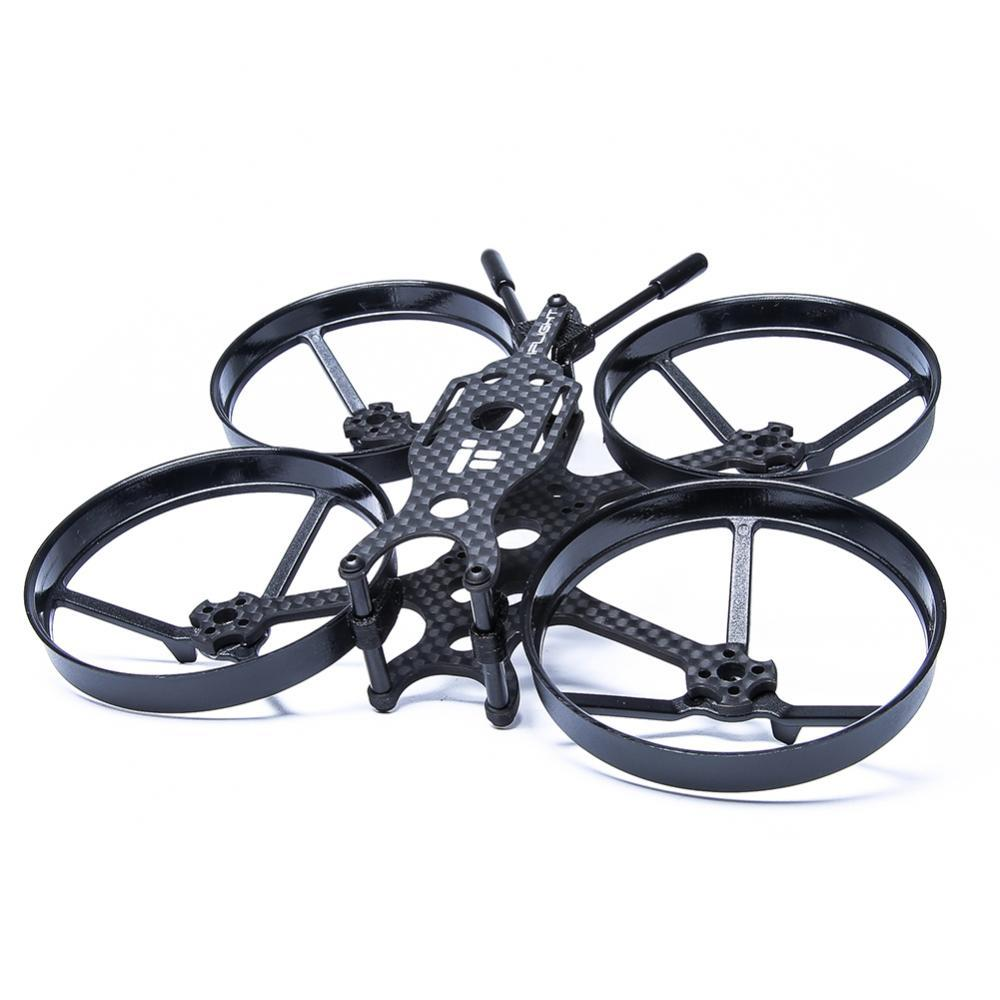
\includegraphics[width=0.5\linewidth]{../RW/pics/frame}
	\caption{Рама для экспериментального образца квадрокоптера
	}
	\label{fig:frame}
\end{figure}

Данная рама используется для создания экспериментального образца. В случае массового производства комплектов, которые будут получены при достижении поставленной цели, рама может быть заменена собственной разработкой.

Перейдем к выбору электроники.

Электроника квадрокоптера должна быть совместимой по характеристикам и габаритам. 

Для управления с наземной станции полетный контроллер должен:
\begin{itemize}
	\item обладать минимум 2 UART портами;
	\item иметь процессор на базе F405 / F745 / F765 чипа.
\end{itemize}

UART (Universal asynchronous receiver / transmitter) -- это аппаратный последовательный интерфейс, который позволяет подключать датчики и периферию к полетному контроллеру. У него есть два вывода для внешнего соединения: TX -- для передачи данных, RX -- для приема.

UART порты потребуются для подключения устройства приема -- передачи телеметрии и возможности подключения дополнительной периферии.

Выбор чипа процессора основан на требованиях к ресурсам по памяти, производительности и периферии. Для того, чтобы прошить PX4, необходим объем памяти процессора не ниже 1 МБ. Такое условие выполняют процессоры на базе F405 / F745 / F765. Преимущество F7 чипов в том, что обеспечивается больше памяти и портов, а также лучше поддерживаются. Но они дороже, выбор полетных контроллеров на таких чипах меньше, а разработка собственного полетного контроллера пока не целесообразна.

Винто -- моторная группа должна быть оптимизирована под задачи автономного полета в помещении на небольшой скорости и устанавливаться в выбранную раму. У моторов бесколлекторного типа основными параметрами являются размеры статора -- неподвижной части мотора (4 цифры) и количество оборотов на вольт (kv). В четырехзначном числе первые два отвечают за диаметр статора, вторые -- за высоту статора. При одинаковых объемах статора крутящий момент на низких оборотах будет больше у того мотора, где больше диаметр статора, а на высоких оборотах там, где больше высота. Для экспериментального образца оптимальным выбором являются моторы 1202. Количество оборотов на вольт выберем, учитывая напряжение аккумулятора. Чем больше напряжение, тем меньше количество оборотов на вольт должно быть на моторе. Каждая ячейка, подключенная последовательно увеличивает напряжение на 4.2 В в заряженном состоянии. Для квадрокоптера с диагональю рамы 120 мм по соотношению вес / токоотдача наиболее выгодно ставить аккумуляторы с 2-3 ячейками. Основываясь на таблице характеристик, приведенных производителем, были выбраны моторы с 6000 kv (рисунок \ref{fig:motor}).
Учитывая потребление тока моторами на полном газу и добавляя 10 -- 15 \% запаса, получаем характеристику регуляторов -- максимальный ток, проходящий через них. На экспериментальном образце он равен 15 А.
\begin{figure}[H]
	\centering
	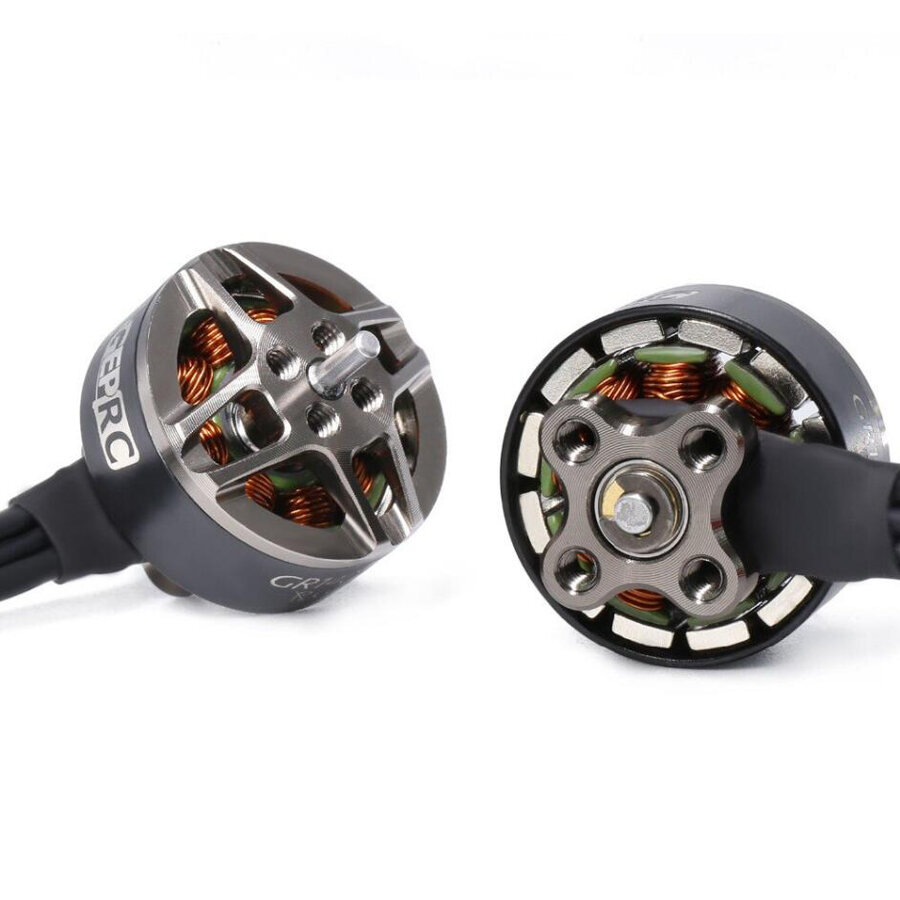
\includegraphics[width=0.5\linewidth]{../RW/pics/motor}
	\caption{Моторы для экспериментального образца квадрокоптера
	}
	\label{fig:motor} % эта метка позволяет ссылаться на рисунок в тексте
\end{figure}

\begin{figure}[H]
	\centering
	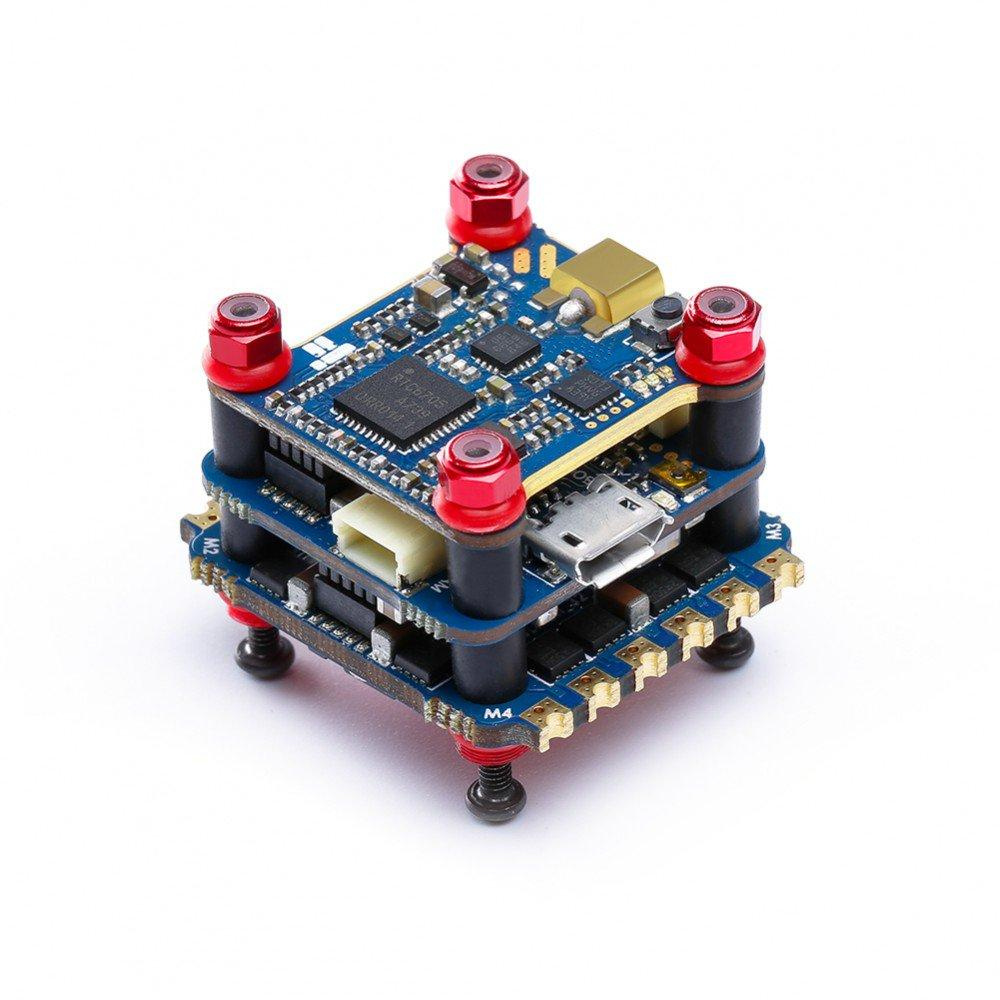
\includegraphics[width=0.5\linewidth]{../RW/pics/stack}
	\caption{Стек электроники для экспериментального образца квадрокоптера
	}
	\label{fig:stack} % эта метка позволяет ссылаться на рисунок в тексте
\end{figure}

Видеопередатчик и камера выбирались исходя из поставленных условий. Видеосигнал аналогового типа дешевле и передается с задержкой меньше, чем цифровой сигнал. MVP решение будем основывать на аналоговом сигнале. Так как необходимо будет передавать видеопоток, камера должна иметь максимально возможное количество телевизионных линий -- разрешающая способность (TVL). Для камер нано формата это 1000 TVL. Размер изображения может быть как 4:3 и 16:9. Формат PAL / NTSC также может быть выбран на усмотрение.

Видеопередатчик обладает такими характеристиками как:
\begin{itemize}
	\item выходная мощность;
	\item выходная частота;
	\item количество каналов.
\end{itemize}

Для помещений мощность 25mW является оптимальной. Количество каналов должно быть выбрано таким образом, чтобы в случае совместных полетов сигнал не пересекался с сигналом другого беспилотника. Современные видеопередатчики имеют 40 каналов. Частота видеосигнала будет использоваться 5.8ГГц.

Для общения с наземной станцией квадрокоптеру понадобятся устройства приема-передачи телеметрии. Протокол, бод-рейт (скорость передачи данных для подключенного устройства приема-передачи данных) и частота устройств станции и квадрокоптера должны совпадать.

Программная часть квадрокоптера полностью осуществляется прошивкой PX4.

%//estimator lpe / ekf
%\url{https://dev.px4.io/v1.9.0/en/ros/offboard\_control.html}
%\url{https://dev.px4.io/v1.9.0/en/ros/external_position_estimation.html}
\subsection{Настройка дрона для передачи телеметрии и видеопотока на наземную станцию}

%\https://discuss.ardupilot.org/t/indoor-autonomous-flight-with-arducopter-ros-and-aruco-boards-detection/34699

\subsubsection{Настройка PX4}
Через конфигуратор qgroundcontrol на полетный контроллер загружается прошивка PX4, после чего необходима первоначальная настройка.

Последовательность действий:
\begin{itemize}
	\item указание прошивке на тип и схему БПЛА (квадрокоптер);
	\item калибровку датчиков (акселерометра, магнитометра, гироскопа...);
	\item проверка корректности ориентации датчиков положения -- акселерометра и гироскопа (отклонения по всем осям происходят в нужные стороны);
	\item конфигурация протокола радиоуправления;
	\item калибровка и настройка каналов радиоуправления (выставлены последовательно соответствующие оси и добавлены необходимые режимы);
	\item проверяется и задается последовательность моторов (порядковые номера моторов соответствуют используемым прошивкой полетного контроллера);
	\item проверяется направление вращений моторов и пропеллеров (диагональные моторы вращаются в одинаковых направлениях согласно выбранной схеме ЛА).
\end{itemize}

Часто в связи с некорректной настройкой одного из описанных пунктов возникают неконтролируемые ситуации при старте -- дрон отказывается взлетать или переворачивается при взлете.

Выставляются полетные режимы:

ACRO -- режим, где отклонением стиков задается угловая скорость для соответствующей оси дрона. Центральное положение стика означает нулевую угловую скорость; в то время как угловая скорость при крайнем положении настраивается значением системы рейтов. Таким образом, при нулевом положении стика дрон не возвращается в горизонт (отсутствует стабилизация уровня). Режим ACRO используется для акробатических полетов, когда требуется плавное и быстрое управление \cite{ardupilot}.

STABILIZED -- режим стабилизации дрона, когда стики аппаратуры находятся в центре; используется для ручного управления в ходе полетных испытаний внутри помещения.

POSHOLD -- удержание позиции по датчикам / компьютерному зрению; когда будет настроена система оценки положения дрона в пространстве, при включении указанного режима дрон должен держаться в одной точке с учетом погрешности.

OFFBOARD -- управление полетом с внешнего компьютера. Этот режим используется для программирования автономных полетов \cite{clover}, при котором управление происходит из выполняемой на внешнем компьютере программы.

После выполнения описанных в начале раздела шагов производится взлет в ручных режимах. Во время полета проверяется ПИД регулирование.

Настройка ПИД-регулятора производится стандартным методом step res\-ponse \cite{tau}. Суть метода заключается в передаче ступенчатого управляющего сигнала на вход регулятора и анализе реакции системы на него.
Медленная реакция на ступенчатый управляющий сигнал указывает на низкий коэффициент пропорциональной составляющей.
Коэффициент увеличивается до появления характерного перерегулирования.
После чего остаточные осцилляции гасятся путем повышения коэффициента дифференциальной составляющей.

Далее изменяются параметры для взаимодействия с Raspberry Pi: указывается используемый порт (UART) и бод-рейт 921600.
Для уменьшения задержки вместо всех mavlink сообщений на наземную станцию будут отправляться только сообщения внешнего визуального позиционирования.

Отключаются использование компаса и GPS, так как они не используются, и выставляются параметры для оценки положения по ECL.

Библиотека оценки и управления (ECL) использует алгоритм расширенного фильтра Калмана (EKF) для обработки измерений датчика и предоставления оценки следующих состояний:
\begin{itemize}
	\item кватернион, определяющий вращение из одной системы отсчета (North, East, Down локальной координатной плоскости) в другую ( X, Y, Z тела);
	\item скорость на IMU - North, East, Down (м / с);
	\item положение в IMU - North, East, Down (м);
	\item оценки смещения угла дельты IMU - X, Y, Z (рад);
	\item оценки смещения дельта-скорости IMU - X, Y, Z (м / с);
	\item компоненты магнитного поля Земли - North, East, Down (гаусс);
	\item смещение магнитного поля рамы кузова автомобиля - X, Y, Z (Гаусс);
	\item скорость ветра - север, восток (м / с).
\end{itemize}

EKF реализует систему <<отложенного временного горизонта слияния>>, что позволяет учесть временные задержки опроса датчиков относительно IMU. Данные для каждого датчика буферизуются FIFO и извлекаются из буфера с помощью EKF для использования в нужное время. Компенсация задержки для каждого датчика регулируется параметрами EKF2*DELAY.

EKF имеет разные режимы работы, которые позволяют использовать различные комбинации опроса датчиков. При запуске фильтр проверяет минимальную жизнеспособную комбинацию датчиков и после завершения начального выравнивания наклона, рыскания и высоты входит в режим, который обеспечивает оценку вращения, вертикальной скорости, вертикального положения, отклонения угла отклонения IMU и отклонения дельта-скорости IMU.

Для этого режима требуются данные IMU, источник рыскания (магнитометр или система внешнего визуального позиционирования (external vision)) и источник данных о высоте. Этот минимальный набор данных требуется для всех режимов работы EKF. Затем данные других датчиков можно использовать для оценки дополнительных состояний \cite{px4}.

В качестве системы внешнего визуального позиционирования используется RPi c камерой.

%https://docs.px4.io/master/en/advanced_config/tuning_the_ecl_ekf.html

%https://docs.px4.io/master/en/ros/external_position_estimation.html
%https://docs.px4.io/master/en/peripherals/mavlink_peripherals.html

\subsubsection{Настройка Raspberry Pi}

Для RPi выбрана операционная система raspbian stretch lite.
%http://www.pcds.fi/downloads/operatingsystem/debianbased/raspbian/archive/stretch/raspbian.stretch.html
С помощью команд, представленных в листинге \ref{lst:5}, был записан образ на карту памяти микрокомпьютера.
\begin{Program}[H]
	\caption{Подготовка карты памяти для RPi} \label{lst:5}
	\begin{MyCode}
	$ unzip -p 2018-11-13-raspbian-stretch-lite.zip
	$ sudo dd if=/home/qw/2018-11-13-raspbian-stretch-lite.img of=/dev/sdd
	$ sync
	\end{MyCode}
Для подключения к роутеру изменены параметры wpa\_supplicant.conf.

	\begin{MyCode}
	$ less /etc/wpa_supplicant/wpa_supplicant.conf
	ctrl_interface=DIR=/var/run/wpa_supplicant GROUP=netdev
	update_config=1
	country=RU
	
	network={
		ssid="ИМЯ_ТОЧКИ_ДОСТУПА"
		psk=passwd
	}
		\end{MyCode}
\end{Program}

%https://habr.com/ru/post/419947/
Для возможности удаленного подключения создан файл ssh в каталоге /boot.

После произведенных шагов карта памяти устанавливается в RPi, и с помощью утилиты nmap на наземной станции проверяются все подключения к роутеру (листинг \ref{lst:6}).
\begin{Program}[H]
	\caption{Поиск адресов в подсети роутера} \label{lst:6}
	\begin{MyCode}
	$ sudo nmap -sn 192.168.1.0/24
	...
	Nmap scan report for 192.168.1.148
	Host is up (-0.062s latency).
	MAC Address: B8:27:EB:D3:B7:09 (Raspberry Pi Foundation)
	Nmap scan report for ikherty (192.168.1.28)
	Host is up.
	Nmap done: 256 IP addresses (4 hosts up) scanned in 4.42 seconds
	...
	\end{MyCode}
\end{Program}

192.168.1.148 -- адрес Raspberry Pi.

%https://www.raspberrypi.org/documentation/remote-access/ip-address.md
Производится удаленное подключение по ssh по найденному адресу, и устанавливаются пакеты gstreamer для запуска трансляции видео с борта дрона.
Для обмена данными между полетным контроллером и RPi устанавливается пакет ser2net и в конфигурационном файле /etc/ser2net.conf добавляется строка, определяющая способ общения, в данном случае она выглядит так (листинг \ref{lst:7}):
\begin{Program}[H]
\caption{Параметры для обмена сообщениями между полетным контроллером и RPi} \label{lst:7}
	\begin{MyCode}
	2000:raw:0:/dev/ttyAMA0:115200 8DATABITS NONE 1STOPBIT
	\end{MyCode}
\end{Program}

Для использования RPi камеры в качестве источника данных трансляции производится сборка gst-rpicamsrc из репозитория \url{https://github.com/thaytan/gst-rpicamsrc} с помощью команд, представленных в листинге \ref{lst:8}:
\begin{Program}[H]
\caption{Сборка rpicamsrc} \label{lst:8}
	\begin{MyCode}
	$ git clone https://github.com/thaytan/gst-rpicamsrc
	$ cd gst-rpicamsrc
	$ make
	$ make install
	\end{MyCode}
\end{Program}

Все необходимые изменения внесены, далее следует произвести настройку наземной станции.

